\section{电气元件}\label{sec:dianqiyuanjian}

{\bfseries 知识目标}
\begin{itemize}
\item 掌握图块的概念
\item 掌握图块的定义、插入、输出方法
\item 掌握图块属性定义与设置知识
\end{itemize}

{\bfseries 技能目标}
\begin{itemize}
\item 能够完成电子元件的定制
\end{itemize}

本任务以绘制\ref{fig:zhumodianlu}所示电路图中的电子元件为目标,主要是帮助读者掌握AutoCAD的图块的概念,以便于在绘图过程中将大量重复的图形定义为图块,以提高图形的绘制速度。

\subsection{电容元件}
首先,让我们来绘制图\ref{fig:zhumodianlu}所示电路图中的电容元件。

第一步,先绘制电容元件的对称中心线。

\noindent
\begin{figure}[htbp]
\centering
\subfloat[]{\label{fig:dianrong1}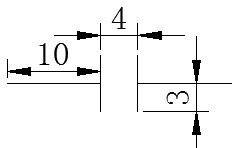
\includegraphics[scale=0.3]{dianrong1.png}}\hspace{20pt}
\subfloat[]{\label{fig:dianrong2}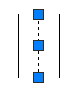
\includegraphics[scale=0.5]{dianrong2.png}}\hspace{20pt}
\subfloat[]{\label{fig:dianrong3}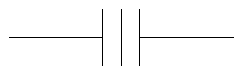
\includegraphics[scale=0.5]{dianrong3.png}}
\subfloat[]{\label{fig:dianrong4}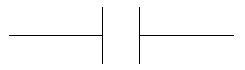
\includegraphics[scale=0.5]{dianrong4.png}}
\caption{电容元件绘制}
\end{figure}

\noindent
命令:line\\
指定第一点:\\
指定下一点或 [放弃(U)]: @6$<90$\\
指定下一点或 [放弃(U)]:\\
\indent

第二步,以对称中心做为偏移对象,向左右各偏移2mm,如图\ref{fig:dianrong2} 所示。

\noindent
命令: offset
当前设置: 删除源=否  图层=源  OFFSETGAPTYPE=0\\
指定偏移距离或 [通过(T)/删除(E)/图层(L)] $<$通过$>$:  2\\
选择要偏移的对象,或 [退出(E)/放弃(U)] $<$退出$>$:\\
指定要偏移的那一侧上的点,或 [退出(E)/多个(M)/放弃(U)] $<$退出$>$:\\
选择要偏移的对象,或 [退出(E)/放弃(U)] $<$退出$>$:\\
指定要偏移的那一侧上的点,或 [退出(E)/多个(M)/放弃(U)] $<$退出$>$:\\
选择要偏移的对象,或 [退出(E)/放弃(U)] $<$退出$>$:\\
\indent

第三步,绘电容接线时,以其最左侧竖线的中心点为起点向左绘制10mm的线条,然后以中心线做另一电容接线,最终结果如图\ref{fig:dianrong3}所示。

\noindent
命令: line\\
指定第一点: mid\\
于\\
指定下一点或 [放弃(U)]: @10$<$-180\\
指定下一点或 [放弃(U)]:\\
命令: mirror\\
选择对象: 找到 1 个\\
选择对象:  指定镜像线的第一点: 指定镜像线的第二点:\\
要删除源对象吗?[是(Y)/否(N)] $<N>:$

\indent
最后,删除中心线,完成电容元件的绘制,其结果如图\ref{fig:dianrong4}所示。

由于电器元件通常都需要重复使用,为了提高我们的绘图速度,需要将绘制的电气元件定义为块并写入文件中,才能够实现其重复利用的目的。下面我们将通过电容块的定义来说明块的定义过程。当我们输入block命令后,会出现图所示的块定义窗体。我们在窗体中命名块的名称为电容,点击拾取点并选择电容元件的最左点来完成基点的定义,点击选择对象并选整个电容图形来完成对象的定义,最后点击确定。

\noindent
命令: block 指定插入基点:\\
选择对象: 指定对角点: 找到 4 个\\
选择对象:\\

\indent
完成块定义后,还需要通过块写命令wblock将定义的块写入dwg文件中才能够实现随时调用和重复利用。
\subsection{接地元件}

\subsection{电阻元件}

\subsection{电灯元件}

\subsection{二极管元件}

\subsection{三极管元件}

\section{触摸延时开关电路图}

\endinput